\newpage
\section{ Теоретические основы }

\subfile{src/common_definitions}
\subfile{src/common_using_symbol}

\newpage
\subsection{ Физические процессы в шаговом двигателе }
Если не учитывать насыщение магнитной системы, то для статического синхронизирующего
момента $M(\theta)$ справедливо равенство \cite[стр. 82]{Chilikin}:

\begin{equation}
\label{step_motor_torque_common}
    M(\theta)
    = \frac{dW_r}{d\theta_m}
    = p \frac{dW_s}{d\theta}
    = \frac{1}{2} p I_s \frac{dL_s}{d\theta}
        + \frac{1}{2} p I_r \frac{dL_r}{d\theta}
        + \frac{1}{2} p I_{s} I_r \frac{dL_{sr}}{d\theta}
\end{equation}

$I_{s}, I_{r}$ - установившееся значение токов статора и ротора соответсвенно

$L_{s}(\theta)$ - индуктивность статора

$L_{r}(\theta)$ - индуктивность ротора

$L_{sr}(\theta)$ - взаимоиндукция ротора и статора

Частота собственных упругих колебаний ротора \cite[гл 3.1]{Chilikin} при малых
отклонениях от положения устойчивого положения позволяет получить сторогую оценку
механической подвижности системы и является ее мерой.

\begin{equation}
\label{step_motor_torque_without_load_and_with_unstable_rotor}
    M(\theta)
    = - M_{m} \sin{\theta}
    = - M_{m} \sin{p\theta_{M}}
\end{equation}

\begin{equation}
\label{step_motor_dynamic_move_equation}
    J \ddot{ \theta_{M} } + M_{m} \sin{p \theta_{M}} = 0
\end{equation}

При малых отклонениях от положения равновесия таких что:
\begin{equation}
    \sin{\theta} \thickapprox 0
\end{equation}

\begin{equation}
    \label{rotor_like_harmonical_oscilator_equation}
    \ddot{\theta} + \frac{p M_{m}}{J} \theta = 0
\end{equation}

\begin{equation}
    \label{friquent_for_rotor_self_oscilating}
    \omega = \sqrt{ \frac{p M_{m}}{J} }
\end{equation}

Процесс изменения тока в обмотке шагового двигателя при ШИМ-управлении \cite[гл. 6.4, стр. 239]{Chilikin}:

Для случая $0 \le \varepsilon \le \zeta$:
\begin{equation}
    \label{winding_current_with_pwm_control_1}
    i[ n; \varepsilon ] = \frac{ U_1 }{ R }
                            \cdot \{ 1
                                     - \frac { e^{ -\sigma \cdot \varepsilon } } { 1 - e^{-\sigma} }
                                            \cdot [ (1 - e^{-n\sigma})
                                                    - e^{ -(1 - \zeta) \cdot \sigma }
                                                        \cdot ( 1 - e^{-n\sigma + \sigma} )
                                                  ]
                                  \}
                        - \frac{ U_2 }{ R }
                            \cdot \frac {e^{-\sigma}} {1 - e^{-\sigma}}
                            \cdot ( 1 - e^{ -n \cdot \sigma + \sigma } )
                            \cdot ( 1 - e^{ -\sigma + \sigma \cdot \zeta } )
\end{equation}

Для случая $\zeta \le \varepsilon \le 1$:
\begin{equation}
    \label{winding_current_with_pwm_control_0}
    i[n; \varepsilon] =
        \frac{ U_{1} + U_{2} }{ R }
            \cdot \frac{ 1 }{ 1 - e^{-\sigma} }
            \cdot (1 - e^{-\sigma\zeta})
            \cdot (1 - e^{-n\sigma})e^{-\sigma\varepsilon + \sigma\zeta}
        - \frac{ U_{2} }{ R }
            \cdot [ 1 - e^{ -( n - 1 + \varepsilon - \zeta ) \sigma } ]
\end{equation}

$\varepsilon = \frac{ t }{ T_\text{ШИМ} }$

$\zeta = \frac{ t_{1} }{ T_\text{ШИМ} }$

$\sigma = \frac{ T }{ T_\text{ШИМ} }$

$T = \frac{ L }{ R }$

$n$ - число периодов импульсов напряжения

$t_{1}$ - время подачи напряжения внутри импульса, с

$T_\text{ШИМ}$ - период ШИМ, с

$t$ - текущее время, с

Максимальное значение тока в импульсе ШИМ согласно (\ref{winding_current_with_pwm_control_1}) при
$\varepsilon=\zeta$ и $U_{2}=0$:

\begin{equation}
    \label{max_current_in_the_n_pwm_pulse}
    i_{max}[n; \zeta] =
        I_{0}
            \cdot \{ 1
                     - \frac{ e^{-\sigma \cdot \zeta} }{ 1 - e^{-\sigma} }
                       \cdot [ (1 - e^{-n\sigma})
                               - e^{ -(1 - \zeta) \cdot \sigma }
                                    \cdot ( 1 - e^{-n\sigma + \sigma} )
                             ]
                  \}
\end{equation}

Где $I_0 = \frac{ U_{1} }{ R }$

Минимальное значение тока в импульсе ШИМ согласно (\ref{winding_current_with_pwm_control_1}) при
$\varepsilon=1$ и $U_{2}=0$:

\begin{equation}
    \label{min_current_in_the_n_pwm_pulse}
    i_{min}[n; \zeta] =
        I_{0}
            \cdot \frac{ 1 }{ 1-e^{-\sigma} }
            \cdot (1 - e^{-\sigma\zeta})
            \cdot (1 - e^{-n\sigma})
            \cdot e^{-\sigma + \sigma\zeta}
\end{equation}

Предел нарастания тока $I_{pwm,max}$ для данного коэффициента заполнения ШИМ получим из
\ref{max_current_in_the_n_pwm_pulse} в пределе при $n \to \infty$

\begin{equation}
    \label{asymptote_of_current_within_constol_pulse}
    I_{pwm,max}[\zeta]=
        \lim_{n \to \infty} i_{max} [n; \zeta] =
            I_{0} \cdot frac{ 1 - e^{-\sigma\zeta} }{ 1 - e^{-\sigma}}
\end{equation}

Скорость нарастания максимумов тока в каждом импульсе оценим как отношение
(\ref{asymptote_of_current_within_constol_pulse}) к (\ref{max_current_in_the_n_pwm_pulse}):

\begin{equation}
    \label{ current_grow_estimate }
    \frac{ i_{max}[n; \zeta] }{ I_{pwm,max}[\zeta] } = 1 - e^{-n \sigma}
\end{equation}

Отсюда мы можем оценить время нарастания тока в течение управляющего импульса:

$$
    n_{ 95 \% } = - \frac{ 1 }{ \sigma }  \cdot \log{(0.05)} \approx \frac{ 3 }{ \sigma }
$$

Передаточная функция шагового двигателя для одного шага при управлении источником
тока \cite[гл. 4.2, ф-ла 4.65]{Kenio}.

\begin{equation}
    \label{step_motor_transfer_function}
    G(s) = \frac{ \omega_{np}^{2} }
                { s^{2} + \frac{D}{J} \cdot s + \omega_{np}^{2} }
\end{equation}

\newpage
\subsubsection{ Управление без ОС }
C помощью (\ref{step_motor_transfer_function}) можно определить пороговую
частоту переключения обмоток, после которой двигатель не сможет запускаться на данной нагрузке.

Собственная частота вращения ротора \cite[гл. 4.2, ф-ла 4.48]{Kenio}

\begin{equation}
    \label{rotor_natural_frequency}
    \omega_{np} = \sqrt{\frac{N_{r}K_{T}I_{o}}{J}}
\end{equation}

Постоянная момента, выраженная из \cite[гл. 4.2, ф-ла 4.52]{Kenio}, при условии
линейности характеристики $r = f(\delta\theta)$

\begin{equation}
    \label{torque_coeff}
    K_{T} = \frac{N_{r}I_{o}\delta\theta}{\tau}
\end{equation}

$N_{r} = 100$ - число зубцов ротора,

$I_{o}$ - ток якоря, А

$\tau$ - статический момент удержания, Н$\cdot$м

$\delta\theta$ - отклонение от положения равновесия, рад.
\newline
\newline

Вычислим $K_{T}$ в положении, в котором момент удержания максимален.
В первом приближении он достигается при отклонении от положения равновесия
$\delta\theta = \frac{\pi}{2}$.

Тогда, подставляя паспортные данные $\tau = 0,9 \text{Н} \cdot \text{м}, I_{o} = 3$
А в (\ref{torque_coeff}), получим:
\begin{equation}
    \label{first_approximation_moment_coeff}
    K_{T} = 2\cdot10^{-3}
\end{equation}

Подставляя (\ref{first_approximation_moment_coeff}) в (\ref{rotor_natural_frequency}), получим:
\begin{equation}
    \label{first_approximation_rotor_natural_frequency}
    \omega_{np} = 1,118 \cdot 10^{2}
\end{equation}

Рассмотрим пусковые возможности двигателя, используя характериистики пускового момента. Очевидно из 
(\ref{step_motor_transfer_function}) пороговая стартовая частота зависит от момента инерции и
статического момента нагрузки.

C некоторым запасом возьмем пусковые характеристики двигателя для данной нагрузки:
$f_{1}, [\text{Гц}]$ - максимальная частота следования импульсов при которой двигатель может и
запускаться и останавливаться без сбое и пропуска шагов взятая с некторым запасом.

\paragraph{Линейное ускорение двигателя}
Если функцию зависимости предельной частоты управления от скорости вращения апроксимировать до
линейной с таким запасом чтоб на графике $f_{max}( \omega )$ она была строго ниже во
всем диапазоне рабочих частот то мы получим закон изменения частоты управления при линейном
ускорении шагового двигателя без выраженной обратной связи. При этом коэффициент наклона этой
наклонной прямой есть ни что иное как предельное ускорение доступное двигателю.
%% формулу надо проверить, в ней что то не так
$$
    f_{max}(t) = f_{1} + \beta_{1} \cdot f_{\text{текущее}}
$$

\paragraph{Линейное торможение двигателя}
Самый простой путь для определения закона управления двигателем при торможении это взять ту же
последовательность что и при ускорении но в обратном порядке.
%% формулу надо проверить, в ней что то не так
$$
    f_{max}(t) = f_{1} + \beta_{2} \cdot f_{\text{текущее}}
$$
Однако, торможение можно выполнять быстрее чем ускорение за счет диссипативных сил,
и коэффициент $\beta_{2}$ несколько больше чем $\beta_{1}$.

\newpage
\subsubsection{ Управление с ОС }
Возможности шагового двигателя могут быть в большой степени расширены при использовании обратной
связи по положению для определения требуемой фазы и времени их включения. В этом случае ШД будет
работать как вентильный двигатель. Управления с ОС предпочтительнее не только потому, что исключает
ошибки в совершении шага. Но и стабилизирует движение ротора, можно достигнуть более высокой
частоты приемистости.

Обратная связь для шагового двишателя в общем виде работает следующим образом:
Пусть шаговый двигатель начинает движение. Оптический датчик определяет положение ротора и передает
информаци логическому блоку, который используя информацию о положении ротора орпеделяет какую фазу
нужно включать для текущего положения и подает на нее питание. Соотношение между настоящим
положением ротора и фазой (или фазами для микрошаговых режимов), которую следует возбудить,
определяется в терминах угла коммутации.
Смена фазы происходит по переходу через целочисленную границу для величины:
$$
    \lfloor ~\theta + \theta_{com}~ \rfloor
$$
Таким образом шаговый двигатель при управлении с обратной связью идентичен вентильному двигателю
постоянного тока.
Частота шагового двигателя с обратной связью определяется величиной нагрузки. Чем больше нагрузка
тем меньше частота врщения.
Угол коммутации предполагает мгновенное нарастание тока в обмотках двигателя, и в таком приближении
угол коммутации при движении в одном направлении можеи изменяться в пределах $[~1,~2)$
Однако на практике одношаговый угол коммутации не используется, так как в этом случае не т
уверенности в продолжении движения, поскольку существует момент трения. Предположим ротор движется к
положению равновесия фазы, возбужденной в данный момент. Очевидно что статический момент действующий
на ротор понижается, то может оказаться так, что момент сухого трения уравняется с моментом
действующим на ротор. В этом случае ротор не дойдет до угла коммутации следующей фазы и
остановится. Двигатель в жтом случае дальше никуда не пойдет. Исходя из этих утвреждений следует
выбирать угол коммутации больше единицы.

Все наши рассуждения предполагали мгновенное нарастание тока.
Но обмотки имеют значительную индуктивность, что вызывает отставание тока по фазе от напряжения.
Тем самым мы должны изменить угол коммутации так, чтобы обеспечить угол равный выбранному углу
коммутации между нарастанием тока и вектором магнитного поля ротора.

\begin{figure}
    \centering
    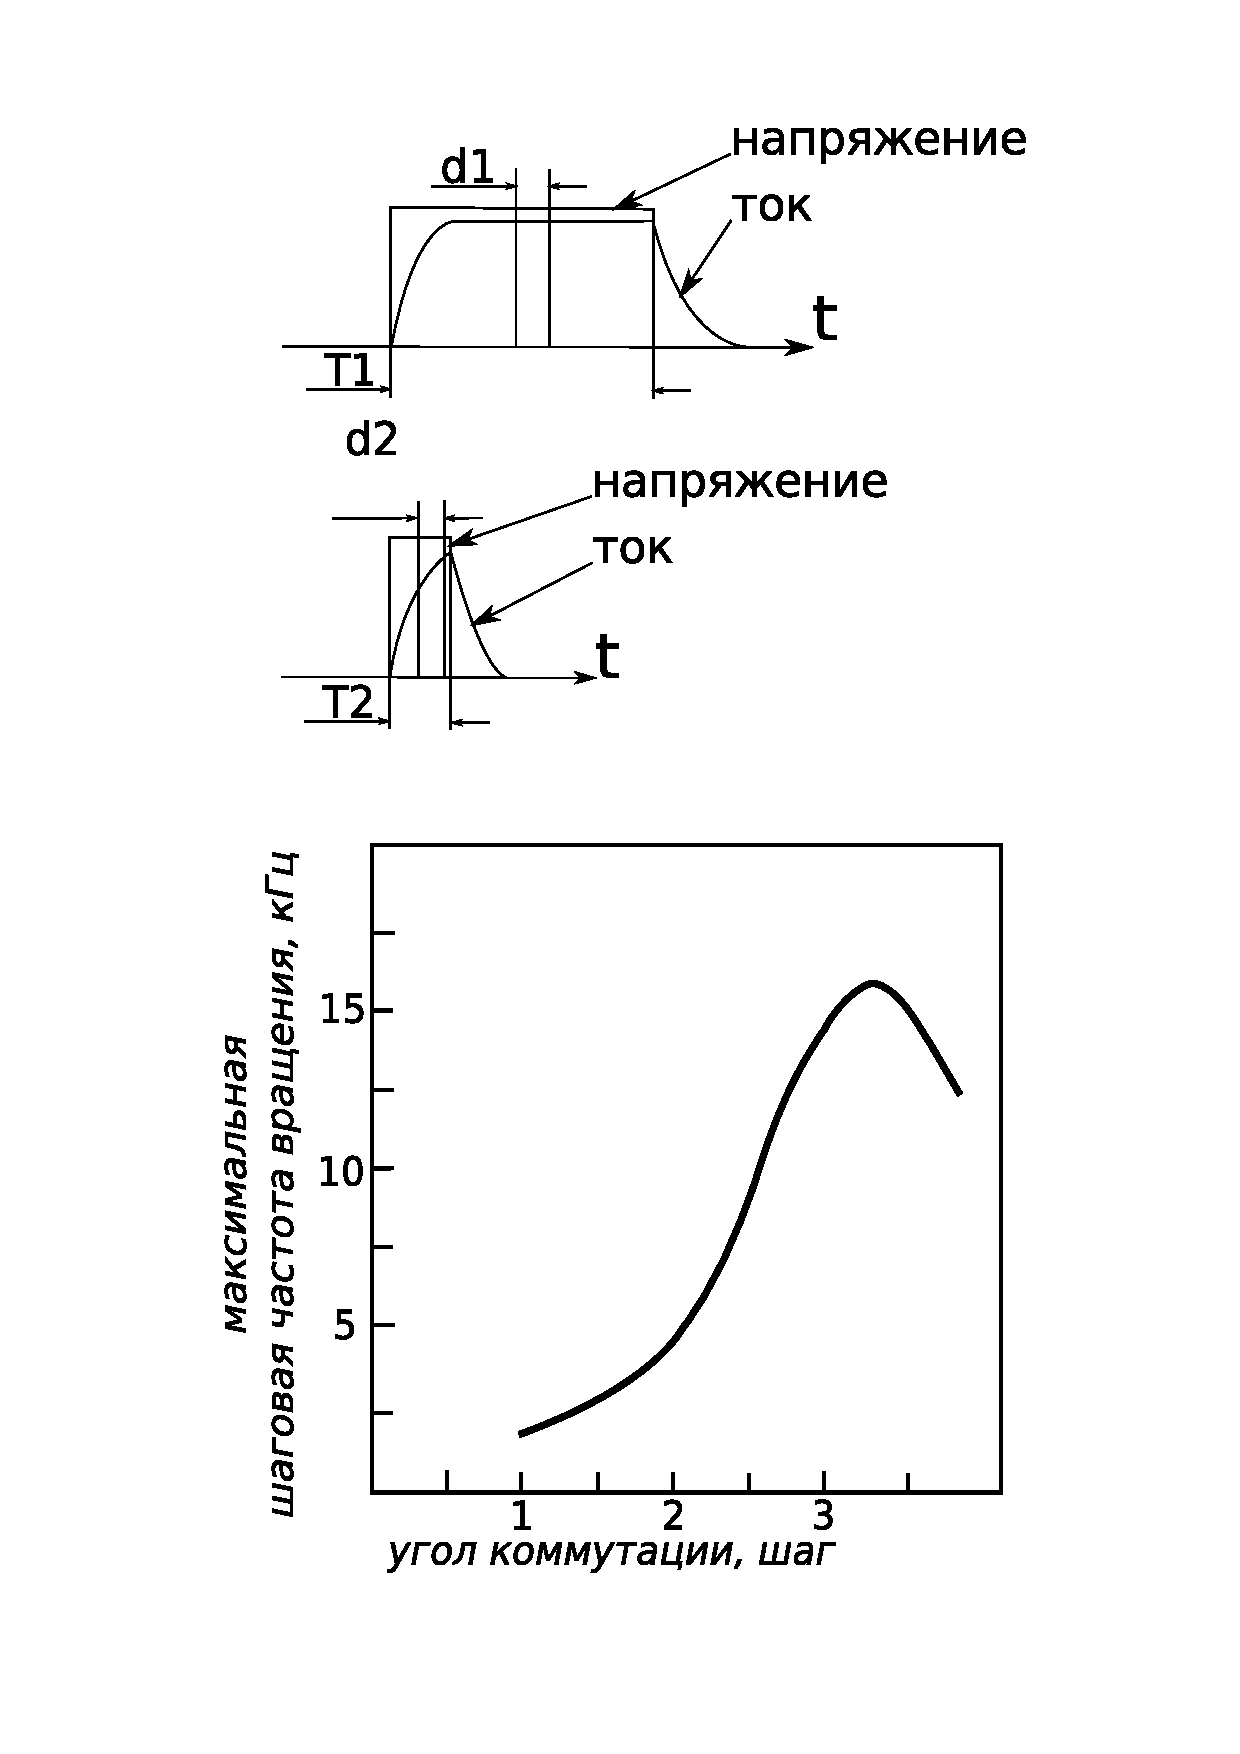
\includegraphics[width=0.7\textwidth, keepaspectratio]{./src/pictures/max_step_motor_by_com_angle}
    \caption{Влияние скорости на параметры управления}
    \label{graph_speed_and_angle_comutation}
\end{figure}

Момент шагового двигателя в зависимости от угла отклонения ротора от положения равновесия:
\begin{equation}
    \label{torque_from_rotor_deviation}
    \tau = K_{T} I_{M} N_{r} ( \theta_{i} - \theta_{0} )
\end{equation}

$K_{T}$ - см. (\ref{torque_coeff})

$I_{M}$ - ток в обмотке, А

$N_{r} = 100$ - число зубцов ротора

$\theta_{0}$ - положение ровновесия, рад.

$\theta_{i}$ - текущее угловое положение, рад.
\newline
\newline

С помощью (\ref{torque_from_rotor_deviation}), задав желаемый угол коммутации и
средний (среднеинтегральный) момент, можно получить значение желаемого среднего
(среднеинтегрального) тока, необходимое для поддержания на данном шаге заданного момента.

Параметризуем угол коммутации и обозначим 
$\theta_{com}$.
Согласно формуле (\ref{torque_from_rotor_deviation}) момент действующий на ротор
в начале импульса управления:

\begin{equation}
    \label{moment_to_rotor_at_the_begin_of_control_pulse}
    \tau_{begin} = K_{T} I_{M} N_{r} ( \theta_{com} )
\end{equation}

в конце импульса:

\begin{equation}
    \label{moment_to_rotor_at_the_end_of_control_pulse}
    \tau_{end} = K_{T} I_{M} N_{r} ( \theta_{com} - \theta_{s} )
\end{equation}

Средний момент для этого участка:
$$
    \tau_{step} = \frac{ \tau_{begin} + \tau_{end} }{ 2 }
$$
$$
    \tau_{step} = K_{T} I_{M} N_{r} ( \theta_{com} - \frac{ \theta_{s} }{ 2 } )
$$

\subsubsection{ Резонансные явления в шаговом двигателе }
Шаговым двигателям свойственен нежелательный эффект, называемый резонансом. Эффект проявляется в
виде внезапного падения момента на некоторых скоростях. Это может привести к пропуску шагов и потере
синхронности. Эффект проявляется в том случае, если частота шагов совпадает с собственной
резонансной частотой ротора двигателя.

При работе двигателя на частоте, совпадающей с резонансной, ротор двигателя колеблется вокруг
положения устойчивого равновесия, возникает провал момента, что приводит к пропуску шагов и потере
синхронности. Без принятия специальных мер шаговый двигатель при разгоне не может пройти резонансную
частоту. Усиление амплитуды колебаний ротора вокруг положения равновесия вызывает сильные вибрации в
передаточных механизмах, что является причиной избыточного шума и приводит к преждевременному износу
механических деталей привода, вибрациям и нарушениям крепления частей и механизмов. В любом случае,
явление резонанса способно существенно ухудшить точностные характеристики привода, поэтому изучение
резонансных явлений и нестабильностей шагового привода представляет большой практический интерес.
\\[5mm]
Опыт показывает \cite[гл. 9]{RatmirovIvobotenko} что, существует 3 вида нестабильности:
\begin{itemize}
    \item Низкочастотный резонанс (частоты $ \le 500 ~\text{Гц}$).
    
    \item Среднечастотная нестабильность. Одна из важнейших проблем, которую пришлось решать при 
            разработке драйвера шагового двигателя и подборе самого двигателя как преодолеть данный
            вид резонанса. Он наблюдается в диапазоне шаговых частот 500 .. 1500 Гц и составляет
            1/4, 1/5 шаговой частоты вращения см. (рис \ref{pic_step_motor_reisonance_plot})

    \item Высокочастотная нестабильность возникает на частотах 1500 .. 2500 Гц, когда двигатель успешно
            проходит область среднечастотной нестабильности.
    
\end{itemize}

\begin{figure}
    \centering
    \includegraphics[width=0.95\textwidth, keepaspectratio]{./src/pictures/step_motor_reisonance_plot}
    \caption{Резонансные частоты среднечастотной нестабильности}
    \label{pic_step_motor_reisonance_plot}
\end{figure}


Самое существенное влияние оказывает среднечастотная нестабильность. Она имеет следующие особенности:
\begin{enumerate}
    \item Колебания имеют одну или несколько частотных компонент. Они не связаны простым соотношением с
            шаговой частотой вращения двигателя и имеют более низкую частоту 5200 Гц.
    
    \item При постоянных условиях работы наблюдаются медленно вырастающие колебания.
            Нарушение нормальной работы системы наступает через несколько секунд или даже минут.
            Возможна внезапная потеря синхронизма.
    
    \item Характеристики нестабильности зависят от схемы и алгоритма управления.
            Существенное влияние оказывает повышение момента инерции системы.
            Большая инерционность увеличивает нестабильность.
\end{enumerate}

Для борьбы с резонансом можно использовать различные методы. Например, применение эластичных
материалов при выполнении механических муфт связи с нагрузкой. Эластичный материал способствует
поглощению энергии в резонансной системе, что приводит к затуханию паразитных колебаний. Другим
способом является применение вязкого трения. Выпускаются специальные демпферы, где
внутри полого цилиндра, заполненного вязкой кремнийорганической смазкой, может вращаться
металлический диск. При вращении этой системы с ускорением диск испытывает вязкое трение, что
эффективно демпфирует систему. 

Существуют электрические методы борьбы с резонансом. Колеблющийся ротор приводит к возникновению в
обмотках статора ЭДС. Если закоротить обмотки, которые на данном шаге не используются, это приведет
к демпфированию резонанса.

И, наконец, существуют методы борьбы с резонансом на уровне алгоритма работы драйвера. Например,
можно использовать тот факт, что при работе с двумя включенными фазами резонансная частота примерно
на $20\%$ выше, чем с одной включенной фазой. Если резонансная частота точно известна, то ее можно
проходить, меняя режим работы.

Если это возможно, при старте и остановке нужно использовать частоты выше резонансной. Увеличение
момента инерции системы ротор-нагрузка уменьшает резонансную частоту.
Самой эффективной мерой для борьбы с резонансом является применение микрошагового режима.

Возможность потери шаговым двигателем устойчивости на резонансных частотах является его существенным
недостатком и требует детального анализа. Результаты анализа должны быть учтены при выборе 
параметроа привода.

